\documentclass[hyperref,english,bachelorofscience,bibnum]{cgvpub}
%weitere Optionen zum Erg�nzen (in eckigen Klammern):
% 
% bibnum	numerische Literaturschl�ssel
% final 	f�r Abgabe	
% lof			Abbildungsverzeichis
% lot			Tabellenverzeichnis
% noproblem	keine Aufgabenstellung
% notoc			kein Inhaltsverzeichnis
% twoside		zweiseitig
\author{Daniel Bekele}
\title{Interactive Registration of 3D Scans in VR}
\birthday{15th January 1995}
\placeofbirth{Jena}
\matno{309845}
\betreuer{Prof. Dr. Stefan Gumhold}
\bibfiles{new_literature_DB}
\problem{
\section{Motivation and Goals:}
When 3D scanning real objects several scans from different views need to be acquired and combined. For high quality reconstruction of a surface model, the relative 3D scanner poses of the different views need to be determined accurately before combining the points from the individual 3D scans. This process is also called registration. The registra-tion problem can be split into coarse and fine registration. In coarse registration a regis-tration with low accuracy is determined which is further refinded by a fine registration, for which fully automatic methods work efficiently. The goal of the thesis is to study the coarse registration problem in an interactive setting where a user adjusts the relative poses in a VR environment and to compare its efficiency with a WIMP based interface, e.g. the one implemented in MeshLab [1].
\section{Tasks:}
\begin{itemize}
\item Literature research on registration approach with a focus on interactive and semi-automatic approaches
\item Collection of a representative set of 3D scan collections
\item Design of a VR environment for the interactive registration realizing the concept of a workbench and a natural alignment of the 3D scan collection that needs to be registered in a way the selection of individual scans is efficient.
\item Implementation of VR-based picking and positioning strategy of individual point clouds based on the interaction capabilities of a VIVE VR set.
\item Development and implementation of a strategy to guide the user through the process of registering all scans of a dataset
\item Integration of an automatic fine registration algorithm like SparseICP [2].
\item Evaluation of the developed methods in a qualitative user study based on a ground truth dataset provided by the Chair of Computer Graphics and Visualization.
\end{itemize}
\section{Optional Tasks:}
\begin{itemize}
\item Integration of a surface reconstruction algorithm in a background process to preview the reconstructed surface based on the current intermediate registration result
\item Design and implement specific interactions and visualizations that help in a faster or more accurate user based registration
\item Improvement of the realism of the VR environment by integrating detailed and textured 3D models.
\end{itemize}
}
\copyrighterklaerung{Hier soll jeder Autor die von ihm eingeholten
Zustimmungen der Copyright-Besitzer angeben bzw. die in Web Press
Rooms angegebenen generellen Konditionen seiner Text- und
Bild"ubernahmen zitieren.}
\acknowledgments{Die Danksagung...}
\abstracten{abstract text english}

\begin{document}
\chapter{3D scan registration}
The registration problem is defined as finding the matching transformation for one or more sets of data to match to a target set of data.(BELEG)
This task can be splitted into the coarse and fine registration.
In order to work properly, or to achieve faster and better results, most registration algorithms require a coarse registration that is done before the actual algorithm starts. 
\begin{quote}
"Depending on the method used, a quite accurate initial
guess is required because some methods have convergence
problems due to the presence of local minima."\cite{salvi2007}
\end{quote}
Fully automated algorithms for the registration problem mostly need 2 different algorithm for coarse and fine alignment. As proposed in a paper by Ji \cite{Ji2017} using an improved method of the ICP for fine alignment and a genetic algorithm for coarse alignment. Other than that Chao uses a semi automatic approach feature based methods. To reduce rotation errors the user decides manually the correct rotation \cite{Chao}

The method proposed by this thesis is a mixture of a manually coarse alignment and simple ICP version that should be capable of running in real time, making it a subject of interest for gaming applictations as well as real time CAD applications.
The coarse registration problem was often solved manually by used a WIMP[explain WIMP] based interface like in Chaos paper \cite{Chao}. To enhance the process further and in order to give the user more insight and controll over his 3D models, a virtual environment is used in our application instead.

The main goal of this thesis is to investigate if this coarse alignment problem can be solved more efficiently by introducing the user to a virtual environment capable of fully displaying the point clouds in all three dimensions, instead of using a WIMP based interface.
The fine registration is then automatically performed by an ICP, in the best case this should execute real time with an animation.

\section{Introduction to registration algorithms}

To achieve this goal of fine registration several steps are necessary:
\begin{enumerate}
\item  Find corresponding points between the roughly aligned sets of data
\item  Find a formula to retrieve the transformation needed to align dataset A to dataset B using the correspondences found in 1.
\item Calculate the actual transformation.
\item Apply the actual transformation
\end{enumerate}

\subsection{Correspondences}

To find corresponding points between 2 sets of points a fast and efficient method is needed, hence the application should work in real time and not use more than 500ms as this is only the first step for the registration algorithm.
The k-nearest neighbour search (knn-search) is commonly used for such problems, as its includes the distances between the nearest points and should deliver good results, given the scans are near together and approximately have the correct rotation. The circumstances of the application fullfill this requirements, since it needs the user to coarse align the scans before the automated fine alignment.
The knn-search does calculate, as its name implies, the distance to the nearest points. To estimate the nearest neighbours, distances between the individual points need to be calculated and then sorted to find the closest points.

Given this situation a simple knn-search with the brute Force method fails. The method would calculate all distances between all points, the resulting complexety of  O(mnd)\cite{Garcia2008}, with m as nubmer of all points from point cloud 1 and n with the number of all points from point cloud 2. d is the number of nearest points that are obtained and stored. This does not meet the requirement of the application to work in real time with point clouds with a higher number of points.
To enhance the efficency of this method many different acceleration data structures have been introduced. The one used in the actual implementation of the application for this thesis is the so called KD-tree.

\subsection{KD-Trees}

\begin{quote}
"k-d trees are a generalization of binary search trees."\cite{Nuchter2007}
\end{quote}
In theory this means that all points are represented by a binary tree structure. The root node contains the whole point cloud. The variable k defines the dimensions which is 3 in our example, hence we are working in 3D space when aligning scans. This variable can be higher if e.g. the colours of scans are as additional information availabe.
Building such a tree has an average rutime in the complexity of O(log n), to optimize it O(n log n)\cite{bentley1975}
Their main advantage is their runtime for knn-querys: 
\begin{quote}
"for nearest neighbor queries [empirically observed average running time of O(log n).]" \cite{bentley1975}
\end{quote}
Using KD-trees for a knn-query results in a much better performance since building a kd tree and using it costs less than using brute force method. Furthermore through parallelization the actual runtime can further be reduced. The code excerpt below shows a snippet which uses a KD-tree for a knn-query executing parallel. This implementation is used during the execution of the fine alignment of the version of the ICP this application uses. The code is taken from the stanford university.

\begin{figure}[htbp]
\begin{lstlisting}[frame=trbl]
           /// Find closest point
           #pragma omp parallel for
            for(int i=0; i<X.cols(); ++i) {
               Q.col(i) = Y.col(kdtree.closest(X.col(i).data()));
           }
\end{lstlisting}
\end{figure}

Newer researches have shown that cached KD-trees algorithms using GPU programming have better results\cite{Garcia2008}, this will not be the case in our application since the GPU is fully occupied by providing a rendered stereoscopic view.

The resulting correspondencies can now be used to calculate a rigid-body transformation that aligns two point clouds. To achieve this, the application uses a commonly known algorithm called Iterative closest point (ICP).

\subsection{The iterative closest point algorithm}

\begin{quote}
"ICP starts with two meshes and an initial guess for their relative rigid-body transform, and iteratively refines the transform by repeatedly generating pairs of corresponding points on the meshes and minimizing an error metric."\cite{Rusinkiewicza}
\end{quote}
In this case the Transformation is a translation and a rotation matrix that when applied to the point cloud aligns it to the target point cloud.

The initial guess is provided by the user with a coarse registration. The ICP then makes use of step 2-4 (see top) always iteratively converging to a local optimum.\cite{Besl92}
The ICP algorithm in the variant that was and is widely used in registration problems and was introduced 1992 by P.J. Besl and Neil D. McKay\cite{Besl92}. Over the years several optimization steps have been added to the ICP in order to boost the speed and efficency.

The variants used by our program is the regular point to point variant using reiterative weighting.
This method uses xxxxxxxx for more stable solutions. Due to problems with the integration of sparse ICP, which uses a more stable error metric the simpler and faster ICP variant has been chosen. This traidoff can lead to NAN or INF results when using the method.
 
Before starting the actual algorithm it has to be considered that the real time requirement can obviously not be fulfilled with larger point clouds as shown in measurements in table 1 [see table with times]. But aligning and grouping several point clouds to one and aligning this greater point cloud will sooner or later result in a large point cloud that has to be aligned. To still fulfill the real time requirement a subsampling method is needed.

\subsection{Subsampling}

The runtime tests as shown in the table show a significant drop rate in runtime when adding too much points. This is especially the case if the point number reach certain limits. We suspect this is the case when the needed storage for the kd trees which lays in O(n * m) [beleg not found] surpasses the computers cache.

To avoid this problem a subsampling method has been introduced, which uses randomized ranged subsampling. Every point cloud of the group of clouds that is aligned to the target group is counted. The resulting number is divided by the subsampling range. The range indicates that every xth point is sampled. The exact point is randomly chosen in between the ranges distance, counting upwards. The resulting subsampled point cloud is now used for the ICP algorithm, reducing the complexity of the actual task by the factor x.

To avoid large overhead due to the creation of randomized numbers the function uses the default and efficient random Microsoft c++ library <random.h> and only array access with offsets. If the ICP is called again with the same point clouds, the application uses the already stored values, further increasing its efficiency.




Below is not part of this work. This are just some tests with the format. dont read it

\section{eine Grafik}
\begin{figure}[htbp]
	\centering
		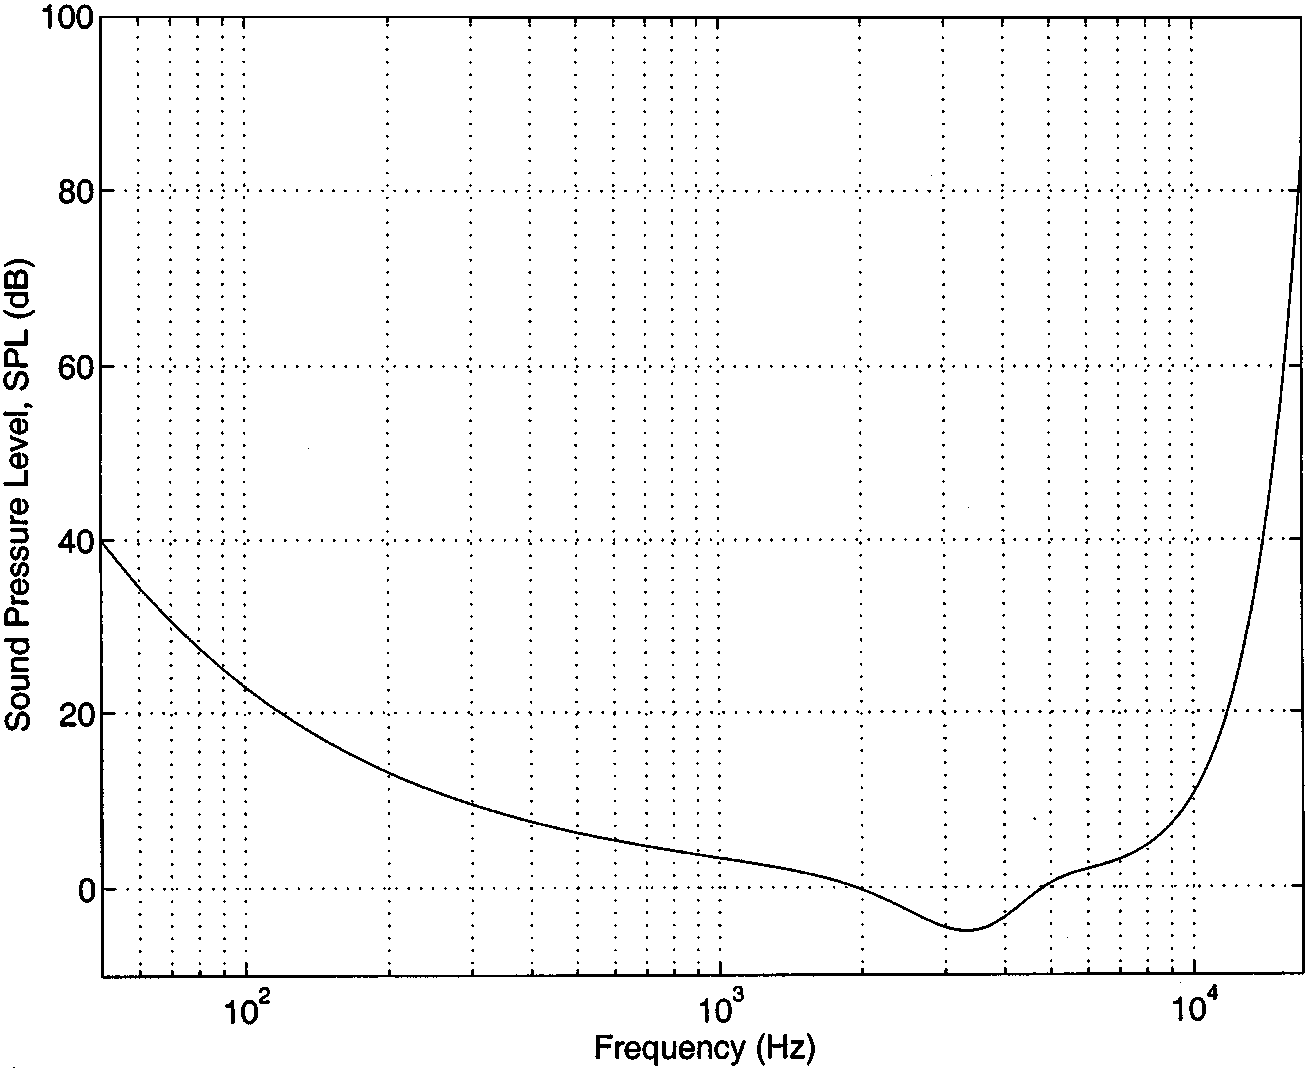
\includegraphics{test.png}
	\caption{beschriftung}
	\label{fig:diplominf}
\end{figure}


\subsection{Etwas Mathe}

\[
\sum_{i=1}^{100}x_i
\]
noch mehr text
\subsubsection{Verweise auf Literatur} 

\paragraph{etwas quelltext}


\begin{figure}[htbp]
\begin{lstlisting}[frame=trbl]
//comment
for(int i = 0; i < 100;i++)
{
test(i);
}
\end{lstlisting}
\end{figure}

text

\cite*{}
\end{document}